\chapter{Rekursion} \label{chp:recursion}
\epigraph{To understand recursion, you must first understand recursion.}{Anonymous}

\begin{wrapfigure}{r}{.3\linewidth}
	\vspace{-10pt}
	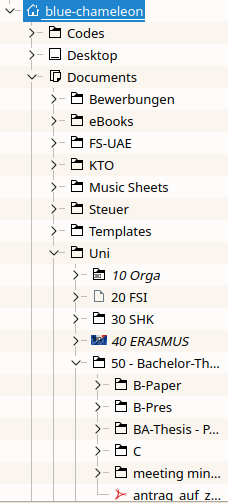
\includegraphics[width=\linewidth]{./gfx/foldertree}
	\caption
	[Auflistung einer Ordnerstruktur]
	{Die Auflistung einer Ordnerstruktur besteht aus Auflistungen von Sub-Ordnerstrukturen}
	\vspace{-90pt}
\end{wrapfigure}
Viele beim Programmieren auftauchende Probleme lassen sich in kleinere Unter-Probleme zerlegen, die dieselbe Form haben wie die ursprünglich zu lösende Aufgabe. Solche zerlegbaren Aufgaben lassen sich so weit aufdröseln, bis man bei einem \emph{elementaren Problem} angekommen ist, das mit einfachen Mitteln zu lösen ist.

Beispiel: Sie wollen die komplette Ordnerstruktur auf Ihrem Rechner auflisten. Dazu müssen Sie, ausgehend von einem Stammverzeichnis, ...
\begin{itemize}
\item alle Dateien des Stammverzeichnisses auflisten
\item alle Ordner im Stammverzeichnis auflisten
\item \emph{die Ordnerstruktur jedes Unterverzeichnisses auflisten}
\end{itemize}

In dieser Auflistung der Teilprobleme finden Sie also eine Unteraufgabe, die gleichlautend mit der ursprünglichen Aufgabe ist: Um eine Ordnerstruktur aufzulisten, müssen Sie eine \emph{Sub}-Ordnerstruktur auflisten. Die Teilaufgabe ist aber \enquote{leichter} als die Lösung des gesamten Problems, da nun nur eine Teilmenge des gesamten Ordnerstruktur aufgezählt werden muss. Schließlich wird man bei einer Teilaufgabe ankommen, die keine Sub-Ordnerstruktur mehr verlangt, da der Ausgangs-Ordner keine Unterordner mehr enthält. Die Auflistung eines solchen Ordners ohne Unterordner ist (verhältnismäßig) einfach.

Wir nennen Probleme, die sich auf gleichförmige Unterprobleme reduzieren lassen \emph{rekursiv}. Die entsprechende Lösungsstrategie nennt sich dementsprechend \emph{Rekursion}.

\section{Funktionen, die sich selbst aufrufen}
Behandeln wir zunächst ein einfaches Beispiel: Wir wollen alle Elemente eines \mintinline{c}{int}-Arrays aufsummieren. Natürlich können wir dies inzwischen schnell mit einer \mintinline{c}{for}-Schleife lösen. Für diesen Abschnitt wollen wir aber eine \emph{rekursive Strategie} wählen:

\begin{center}
\begin{minipage}{.8\linewidth}
\emph{Die Summe aller Elemente einer Liste ist gleich dem ersten Listenelement plus der Summe der verbleibenden Liste ohne ihr erstes Element.}
\end{minipage}
\end{center}

Diese Aufgabe ist direkt lösbar, wenn die verbleibende Liste nur ein Element hat. Ansonsten erkennen wir wieder die rekursive Struktur des Problems.

Zur Lösung setzen wir eine Funktion an, die als Parameter einen Pointer auf den Listenanfang sowie die Länge der Liste erwartet. Diese Funktion wird \emph{sich selbst aufrufen}, also \emph{in die Rekursion gehen}.

\begin{codebox}[Beispiel: Rekursives Aufsummieren]
\begin{minted}[linenos]{c}
#include <stdio.h>

int listsum_recursive(int * list, unsigned int N) {
  if        (N == 1) {
    return list[0];
    
  } else if (N == 2) {
    return list[0] + list[1];
    
  } else {
    return list[0] + listsum_recursive(list + 1, N - 1);
  }
}

int main () {
  int list[] = {1, 2, 3, 4, 5, 6, 7, 8, 9};
  
  printf("Summe: %d\n", listsum_recursive(list, sizeof(list) / sizeof(*list)));
  return 0;
}
\end{minted}
\end{codebox}

\begin{cmdbox}[Ausgabebeispiel: Rekursives Aufsummieren]
Summe: 45
\end{cmdbox}

Wie nun funktioniert dieses Verfahren?

Die Zeilen 1 bis 8 sind unkompliziert. Der Fall einer Liste mit nur einem bzw. zwei Elementen wird mit elementaren Mitteln bearbeitet. Für den interessanten Fall, dass die Unterliste mehr als ein Element hat (\mintinline{c}{else} in Zeile 10) beschreiben wir die Rekursionsstrategie: Wir addieren das erste Listenelement \texttt{list[0]} zur Summe der Unterliste ohne dieses erste Element. Der Ausdruck \texttt{list + 1} beschreibt einen \mintinline{c}{int}-Pointer, der um ein \mintinline{c}{int}-Element gegenüber der ursprünglichen Liste verschoben ist. \texttt{list + 1} zeigt also auf eine \enquote{neue} Liste, die mit dem \emph{zweiten} Element von \texttt{list} beginnt.

In der Umsetzung werden in Zeile 11 die beiden Summanden getrennt voneinander ausgewertet. Das heißt, der Rechner liest den Wert \texttt{list[0]} aus dem Speicher. Die Auswertung des zweiten Summanden sieht (\emph{in Pseudo-Syntax, \ie in nicht gültigem C-Code!}) so aus:

\begin{codebox}[Auswertung: Rekursionsstufe 0 in Pseudosyntax]
\begin{minted}{c}
    return 1 + listsum_recursive({2, 3, 4, 5, 6, 7, 8, 9}, 8);
\end{minted}
\end{codebox}

Als \texttt{Rekursionstiefe} oder \emph{Rekursionsebene} bezeichen wir die Anzahl der \enquote{verschachtelten} Aufrufe. Da wir aus der Funktion \texttt{listsum\_recursive} wieder dieselbe Funktion \texttt{listsum\_recursive} aufrufen, haben wir also gerade Rekursionsebene 1 erreicht.

Natürlich muss jetzt noch der Funktionsaufruf von \texttt{listsum\_recursive} aufgelöst werden. Dies geschieht nach demselben Prinzip wie schon der erste Aufruf, der von der \texttt{main} aus gestartet wurde. Wir gehen also wieder eine Rekursionsebene tiefer, wenn wir wieder auf Zeile 11 treffen. Die Zeile wird dann ausgewertet zu:

\begin{codebox}[Auswertung: Rekursionsstufe 1 in Pseudosyntax]
\begin{minted}{c}
    return 2 + listsum_recursive({3, 4, 5, 6, 7, 8, 9}, 7);
\end{minted}
\end{codebox}

Auch wenn wir immer dieselbe Funktion aufgerufen, wird jeweils ein neuer Scope betreten. Die Bezeichner \texttt{N} und \texttt{list} stehen also auf jeder Rekursions-Ebene für andere Speicherstellen. Sie können sich dies wie verschachtelte Boxen:

\begin{codebox}[Rekursionsstufe 0: Symbol und Werte]
N = 9, list = \{1, 2, 3, 4, 5, 6, 7, 8 ,9\}
\begin{codebox}[Rekursionsstufe 1: Symbole und Werte]
N = 8, list = \{2, 3, 4, 5, 6, 7, 8 ,9\}
\begin{codebox}[Rekursionsstufe 2: Symbole und Werte]
N = 7, list = \{3, 4, 5, 6, 7, 8 ,9\}
\begin{codebox}[Rekursionsstufe 3-6]
...
\begin{codebox}[Rekursionsstufe 7: Symbole und Werte]
N = 2, list = \{8, 9\}
\end{codebox}
\end{codebox}
\end{codebox}
\end{codebox}
\end{codebox}

Obwohl wir formell in derselben Funktion bleiben, hat das Symbol \texttt{N} in Ebene 7 und Ebene 6 nichts miteinander zu tun. Dasselbe gilt für das Symbol \texttt{list}.

In Ebene 7 treffen wir endlich auf einen Fall, den unser Algorithmus ohne weiteren Rekursionsschritt auskommt. Es wird die Summe \texttt{8 + 9} berechnet und zurück gegeben. Dieser Rückgabewert wird nun in Zeile 11 der jeweils übergeordneten Rekursionsebene eingesetzt, um auch dort einen Rückgabewert zu berechnen. Der Stapel wird sozusagen \emph{von innen heraus} aufgelöst:

\begin{codebox}[Rekursionsstufe 0: Rückgabewerte]
\begin{codebox}[Rekursionsstufe 1: Rückgabewerte]
\begin{codebox}[Rekursionsstufe 2: Rückgabewerte]
\begin{codebox}[Rekursionsstufe 3-6]
\begin{codebox}[Rekursionsstufe 7: Rückgabewerte]
return 8 + 9;
\end{codebox}
...
\end{codebox}
return 3 + 39;
\end{codebox}
return 2 + 42;
\end{codebox}
return 1 + 44;
\end{codebox}

\begin{warnbox}[Pseudocode und tatsächliche Werte]
Im obigen Beispiel wurde der Anschaulichkeit halber \texttt{list} mit einer Menge von Werten ersetzt (Darstellung in \{geschweiften Klammern\}). Dies ist keine gültige C-Syntax!

In der Realität wird jeweils ein \emph{Pointer} an die untergeordnete Rekursionsebene weitergeleitet. Alle diese Pointer zeigen auf \emph{überlappende} Speicherbereiche, sind aber jeweils um die Speicherbreite einer Zahl gegeneinander verschoben. Da man nun verschiedene Speicherpunkte als Listen-Anfang interpretiert, und zugleich die Listenlänge \texttt{N} in jeder Rekursionsebene um 1 reduziert, ergeben sich effektiv die oben gezeigten Listen.

Während die oben gewählte Darstellung die Vorgänge klarer macht, sollten Sie sich bewusst sein, was tatsächlich im Speicher abgelegt wird.
\end{warnbox}

\section{Kommunikation über Rekursionsebenen hinweg}
Wie üblich bei Funktionsaufrufen können Sie Werte zwischen den Rekursionsebenen austauschen, indem Sie diese als Parameter übergeben. Dies ist aber nicht immer wünschenswert. Stellen Sie sich etwa vor, Sie wollen eine Sicherheitssperre einbauen und die Rekursionstiefe auf 10 begrenzen. Dies ist möglich über folgenden Ansatz:

\begin{codebox}[Beispiel: Rekunsionstiefe mit Parameter]
\begin{minted}[linenos]{c}
int recursiveFunc(unsigned int depth) {
  if (depth > 10) {return 0;}
  
  depth++;
  recursiveFunc(depth)
  
  // nützlicher Code...
  
  return 1;
}
\end{minted}
\end{codebox}

Allerdings müssen Sie hier beim Aufruf der Funktion \texttt{recursiveFunc} (\eg aus der \texttt{main} heraus) den dort bedeutungslosen Parameter \texttt{depth} angeben. Um dem zu entgehen, können Sie auch das Schlüsselwort \mintinline{c}{static} benutzen.

Wie Sie noch aus Abschnitt \ref{sec:staticVar} wissen, sorgt \mintinline{c}{static} dafür, dass die Speicherzelle für ein so deklariertes Symbol nicht freigegeben wird, wenn die Funktion verlassen wird, dass also der Wert des Symbols zwischen Funktionsaufrufen erhalten bleibt. In diesem Fall bedeutet das also, dass der Wert eines \mintinline{c}{static} Symbols auch über die Rekursionsebenen hinweg erhalten bleibt. Somit können wir das obige Beispiel auch \emph{ohne} Parameter umsetzen:

\begin{codebox}[Beispiel: Rekunsionstiefe ohne Parameter]
\begin{minted}[linenos]{c}
int recursiveFunc() {
  static int depth = 0;
  
  if (depth > 10) {return 0;}
  
  depth++;
  recursiveFunc()
  depth--;
  
  // nützlicher Code...
  
  return 1;
}
\end{minted}
\end{codebox}

Zeile 2 -- die Deklaration und Wertzuweisung von \texttt{depth} wird nur ein einziges Mal\footnote{und tatsächlich bereits zur Kompilierzeit} ausgeführt. Ab dann greift \texttt{depth} von jeder Rekursionsebene auf \emph{dieselbe} Speicherstelle zu. Die Verwendung ist also ähnlich einer globalen Variablen, die aber nur innerhalb von \texttt{recursiveFunc} \enquote{sichtbar} ist.

\section{Laufzeitverhalten von rekursiven Methoden}
Wie Sie wissen, bedeuten Funktionsaufrufe einigen Verwaltungsaufwand, der in Summe spürbar Zeit kosten kann. Hinzu kommt, dass die maximale Rekursionstiefe begrenzt ist, da für jeden Rekursionsschritt gespeichert werden muss, wo die Programmausführung nach Ende eines Rekursionsschritts fortgesetzt werden soll. Diese \emph{Rücksprung-Adresse} wird auf dem Stack abgelegt, der nur begrenzt Speicherplatz anbietet. Zu viele Rekursionsebenen\footnote{mehrere hundert} führen zu einem sogenannten \emph{Stack overflow}.

Es lässt sich beweisen, dass jeder \emph{rekursive Algorithmus} sich auch in verschachtelten Schleifen schreiben lässt. Wo dies \emph{einfach} möglich ist, ist eine solche Lösung ohne Rekursion auch zu bevorzugen. Das obige Beispiel der Summe über ein Array sollte also aus Effizienzgründen besser so implementiert werden:

\begin{codebox}[Beispiel: Iteratives Aufsummieren]
\begin{minted}[linenos]{c}
#include <stdio.h>

int listsum_iterative(int * list, unsigned int N) {
  int reVal = 0;
  
  for (unsigned int i=0; i<N; i++) {
    reVal += list[i];
  }
  
  return reVal;
}

int main () {
  int list[] = {1, 2, 3, 4, 5, 6, 7, 8, 9};
  
  printf("Summe: %d\n", listsum_iterative(list, sizeof(list) / sizeof(*list)));
  return 0;
}
\end{minted}
\end{codebox}

Häufig macht eine rekursive Formulierung den Algorithmus aber für \emph{Menschen} leichter verständlich, und damit auch besser wartbar, erweiterbar oder anpassbar. Dies gilt insbesondere dann, wenn die Problembeschreibung bereits rekursive Elemente enthält, bzw. wenn sich die Aufgabe in \emph{Hierarchie-Ebenen} einteilen lässt. Im folgenden Abschnitt werde ich Ihnen eine rekursive Lösung zum Beispiel am Anfang des Kapitels zeigen. Ich lade Sie dazu ein, diese Lösung in eine nicht-rekursive Form umzuschreiben.

\section{Beispiel: Rekursives Auflisten der Ordnerstruktur}
Der folgende Code ist länger und verwendet einige Befehle, die hier noch nicht besprochen wurden. Sie werden aber feststellen, dass Sie inzwischen die Funktionsweise des Codes erfassen können, auch wenn Sie nicht jedes Detail verstehen. Die Namen der einzelnen Symbole sind dabei so gewählt, dass Ihnen das Verständnis erleichtert wird, wie es auch allgemein gute Praxis ist. Kommentare ergänzen dabei schwerer erfassbare Elemente in knapper Form.

Beginnen Sie beim Nachvollziehen mit der Funktion \texttt{showtree} ab Zeile 186. Diese enthält die Rekursion und ist für dieses Kapitel die interessanteste Funktion. Die Funktion \texttt{print\_indented} ab Zeile 178 sollte Ihnen keine Probleme bereiten.

Fahren Sie dann fort mit der Definition von \texttt{stringlist} und den zugeordneten Funktionen \texttt{make\_stringlist}, \texttt{free\_stringlist}, \texttt{append\_to\_stringlist}, 
\texttt{get\_stringlist\_item} und \texttt{get\_stringlist\_length} in der abgedruckten Reihenfolge. Diese führen einen eigenen Datentyp mit zugehörigen Funktionen ein und illustrieren eine gängige Herangehensweise in der Programmiertechnik: in ihren Eigenschaften eine Einheit bildene Informationen werden zu einem \emph{Objekt} zusammengefasst. Die daran auftretenden Aufgaben werden von allgemein gefassten \emph{Methoden} (Funktionen) erledigt\footnote{Man spricht auch von \emph{Reifikation}, oder \enquote{Verdinglichung}. In Kursen zur \emph{Objektorientierten} Programmierung wie in C++ ist dies ein zentrales Konzept}.

Die Funktion \texttt{get\_directory\_entries} ist auf Anhieb vermutlich schwer zu erfassen, da hier die meisten bisher unbekannten Befehle auftauchen. Ich werde nach dem Code einige Erläuterungen dazu geben. Versuchen Sie aber zuerst, die Zusammenhänge selbst zu erahnen.

\subsection{Code}
\begin{codebox}[Beispielprogramm: \texttt{tree.c}]
\begin{minted}[linenos]{c}
#define _GNU_SOURCE       // use all features from unistd.h

#include <stdio.h>
#include <stdlib.h>
#include <string.h>
#include <unistd.h>       // some file system functions...
#include <dirent.h>       // ... and some more ...
#include <sys/stat.h>     // ... and even more.

// ========================================================================= //
// handle a list of strings

typedef struct {
  unsigned int N;       // number of strings in the list
  char **      items;   // the list itself
} * stringlist;

// ------------------------------------------------------------------------- //

stringlist make_stringlist() {
  /* Create a well-defined initial state so that the other methods don't have
   * to do excessive error-checking
   */
  
  stringlist reVal = malloc(sizeof(stringlist));
  
  if (reVal) {
    reVal->N     = 0;
    reVal->items = NULL;
  } else {
    printf("Error in make_stringlist: Could not allocate memory.\n");
    return NULL;
  }
  
  return reVal;
}

// ......................................................................... //
\end{minted}
\end{codebox}

\begin{codebox}[]
\begin{minted}[linenos, firstnumber=last]{c}
void free_stringlist(const stringlist list) {
  /* frees all memory occupied by the components of a stringlist.
   */
  
  // first, free the items themselves
  for (unsigned int i=0; i<list->N; i++) {
    if (list->items[i]) {free(list->items[i]);}
  }
  
  // then free the list of items
  free(list->items);
  
  // and finally, free the struct
  free(list);
}

// ......................................................................... //

int append_to_stringlist(const stringlist list, const char * item) {
  /* adds an item to the end of a stringlist.
   * returns number of items in the list on success or -1 on failure.
   */
  
  // check whether a NULL pointer was passed
  if (!list) {
    printf("Error in append_to_stringlist: Invalid list.\n");
    return -1;
  }
  
  // make a copy of the item to be added to the list
  char * newItem = malloc(strlen(item) + 1);
  if (!newItem) {
    printf("Error in append_to_stringlist: Not enough memory for new item.\n");
    return -1;
  }
  strcpy(newItem, item);
  
  // make the list one item longer
  char ** longerList = realloc(list->items, (list->N+1) * sizeof(*longerList));
  if (!longerList) {
    printf("Error in append_to_stringlist: Could not expand list.\n");
    free(newItem);
    return -1;
  }
  
  list->items = longerList;
  list->items[list->N] = newItem;
  
  return ++list->N;
}

// ......................................................................... //
\end{minted}
\end{codebox}

\begin{codebox}[]
\begin{minted}[linenos, firstnumber=last]{c}
char * get_stringlist_item(const stringlist list, const unsigned int i) {
  /* access to stringlist items with error checks
   */
  
  // check whether a NULL pointer was passed
  if (!list) {
    printf("Error in get_stringlist_item: Invalid list.\n");
    return NULL;
  }
  
  // check if index out of boundaries
  if (i < list->N) {
    return list->items[i];
    
  } else {
    printf("Error in get_stringlist_item: Invalid index.\n");
    return NULL;
  }
}

// ......................................................................... //

unsigned int get_stringlist_length(const stringlist list) {
  if (!list) {
    printf("Error in get_stringlist_length: Invalid list.\n");
    return 0;
  }
  
  return list->N;
}

// ========================================================================= //
// create lists of files and directories in the current working directory

typedef enum {listtype_files, listtype_directories} listtypes;

stringlist get_directory_entries (const listtypes type) {
  stringlist reVal = make_stringlist();
  
  DIR * filesystem_handle = opendir(".");
      // "." represents current work directory
      // opendir returns NULL if it couldn't open the directory 
  
  struct dirent * directory_entry;
      // will hold name of one item in the directory
  struct stat     statbuffer;
      // will hold kind of one item in the directory (file or folder)
  
  if (filesystem_handle == NULL) {
    printf("Error in get_subdirectories: Could not open current directory\n");
    free_stringlist(reVal);
    return NULL;
  }
\end{minted}
\end{codebox}

\begin{codebox}[]
\begin{minted}[linenos, firstnumber=last]{c}
  // read new entries from the directory as long as there are any.
  while (  (directory_entry = readdir(filesystem_handle)) != NULL  ) {
    // skip special file system elements
    if ((strcmp(directory_entry->d_name, "." ) == 0) ||
        (strcmp(directory_entry->d_name, "..") == 0)
    ) {continue;}
    
    // analyze type of directory enty
    if(  stat(directory_entry->d_name, &statbuffer) == -1  ) {
      printf("Error in get_subdirectories: "
             "Could not determine kind of entry %s\n", 
             directory_entry->d_name);
      free_stringlist(reVal);
      return NULL;
    }
    
    int entry_is_directory = S_ISDIR(statbuffer.st_mode);
    int condition_to_add =
       ( entry_is_directory && (type == listtype_directories)) ||
       (!entry_is_directory && (type == listtype_files      ));
    
    if (condition_to_add) {
      append_to_stringlist(reVal, directory_entry->d_name);
    }
    
  }
  
  closedir(filesystem_handle);
  return reVal;
}

// ========================================================================= //
// recursive traversal of file system

void print_indented(const char * text, const unsigned int n) {
  for (unsigned int i=0; i<n; i++) {printf("  ");}
  
  printf("%s\n", text);
}

// ------------------------------------------------------------------------- //

void showtree(char * startDir) {
  static unsigned int indent_level = 0;
  int                 flag_free_startDir = 0;
  
  if (!startDir) {
    // use current work directory if nothing else was specified.
    startDir = get_current_dir_name();
        // this function uses malloc, thus a free() is needed later
    flag_free_startDir = 1;
        // store information: free is needed.
  }
\end{minted}
\end{codebox}

\begin{codebox}[]
\begin{minted}[linenos, firstnumber=last]{c}
  if (  chdir(startDir)  ) {
    // switch to directory startDir. Return 0 on success, -1 otherwise
    
    printf("\x1b[91m");   // switch to colour red for error output
    print_indented("(invalid directory)", indent_level);
    printf("\033[m");     // restore normal colours
    if (flag_free_startDir) {free(startDir);}
    return;
  }
  
  printf("\x1b[96m");   // show directories in bright cyan
  print_indented(startDir, indent_level);
  printf("\033[m");     // restore normal colours
  
  // get list of directories and go into recursion
  stringlist subdirs = get_directory_entries(listtype_directories);
  if (subdirs) {
    for (unsigned int i=0; i<get_stringlist_length(subdirs); i++) {
      indent_level++;
      showtree(get_stringlist_item(subdirs, i));
      chdir("..");
      indent_level--;
    }
    free_stringlist(subdirs);
  }
  
  // get list of files
  stringlist files = get_directory_entries(listtype_files);
  if (files) {
    for (unsigned int i=0; i<get_stringlist_length(files); i++) {
      print_indented(get_stringlist_item(files, i), indent_level + 1);
    }
    free_stringlist(files);
  }
  
  if (flag_free_startDir) {free(startDir);}
}

// ========================================================================= //

int main (int argc, char ** argv) {
  if (argc) {showtree(argv[1]);}
  else      {showtree(NULL   );}
}
\end{minted}
\end{codebox}

\subsection{Anmerkungen zu \texttt{showtree}}
Als Parameter wird dieser Funktion ein \mintinline{c}{char *} übergeben, also ein String. Dieser benennt das Ausgangsverzeichnis, von dem ab die Auflistung der Ordnerstruktur beginnen soll. Neben einem \enquote{sinnvollen} Pointer auf eine echte Zeichenkette kann aber auch der Wert \texttt{NULL} übergeben werden. In diesem speziellen Fall wird der Rechner angewiesen, vom aktuellen Arbeitsverzeichnis auszugehen. Der Name desselben wird mit der Funktion \texttt{get\_current\_dir\_name} ermittelt. Die Funktion ist im Header \texttt{<unistd.h>} deklariert, sobald das Macro \texttt{\_GNU\_SOURCE} definiert wird.

Wie Sie unter \url{http://man7.org/linux/man-pages/man3/getcwd.3.html} nachlesen können, reserviert \texttt{get\_current\_dir\_name} für den Namen des aktuellen Arbeitsverzeichnisses Speicher, der später wieder mit \texttt{free} freigegeben werden muss. Wir \emph{setzen ein Flag}, \ie speichern die Information, dass wir dieses \texttt{free} später noch ausführen müssen in einer Variablen \texttt{flag\_free\_startDir}.

Die \mintinline{c}{static unsigned int indent_level} speichert die gegenwärtige Rekursionstiefe. Wir benutzen diese Information auch, um damit Einrückungen zu machen, und die hierarchische Struktur des Ordnersystems grafisch wiedergeben.

In Zeile 197 wird \texttt{chdir} aufgerufen. Auch diese Funktion ist im Header \texttt{<unistd.h>} deklariert, und setzt ein neues Arbeitsverzeichnis. Da \texttt{startDir} auch auf \enquote{unsinnige} Strings zeigen kann, ist es möglich, dass dieser Verzeichniswechsel fehlschlägt. In diesem Fall ist der Rückgabewert von \texttt{chdir} gleich \texttt{-1}\footnote{Daneben sind auch andere Wege möglich, wegen derer der Verzeichniswechsel fehlschlagen kann. Beispielsweise kann der Zugriff auf einzelne Verzeichnisse nur dem Administrator gestattet sein, oder ein Netzlaufwerk ist wegen schlechter Verbindung zeitweise nicht erreichbar.}.
Lesen Sie hierzu mehr unter \url{http://man7.org/linux/man-pages/man2/chdir.2.html}.

Beachten Sie Zeile 201: Obwohl wir die Funktion \texttt{print\_indented} bislang noch nicht besprochen haben, dürften Sie intuitiv erfassen, was hier geschieht: Der Text \texttt{(invalid directory)} wird auf dem Bildschirm ausgegeben, und zwar mit einer Einrückung, die der aktuellen Tiefe im Ordnerbaum entspricht. Dass der Effekt ohne genauere Betrachtungen erfasst werden kann ist eine Konsequenz aus der sinnvollen Benennung von Funktionen und Variablen.

Ähnlich verhält es sich mit Zeile 212:
\begin{center}
\mintinline{c}{stringlist subdirs = get_directory_entries(listtype_directories);}
\end{center}
Eine neue Variable vom Typ \texttt{stringlist} mit Namen \texttt{subdirs} wird angelegt und speichert nun den Wert, der von \texttt{get\_directory\_entries(listtype\_directories)} berechnet wurde. Obwohl wir bislang weder wissen, wie dieser Typ \texttt{stringlist} aufgebaut ist, noch wie exakt 
\texttt{get\_directory\_entries} funktioniert, können wir diese Zeile \emph{semantisch} erfassen: gespeichert werden alle Einträge des aktuellen Arbeitsverzeichnisses, die dem 
\texttt{listtype\_directories} entsprechen, also alle Unterordner des aktuellen Arbeitsverzeichnisses.

Wenn diese \texttt{stringlist} nicht leer war (Zeile 213), so wird jedes Element der Liste abgearbeitet. Da dies bei Unterordnern bedeutet, dass wir eine Ebene tiefer in die Rekursion gehen, erhöhen wir zuerst den Zähler \texttt{indent\_level}, bevor wir rekursiv wieder \texttt{showtree} aufrufen. Statt im aktuellen Arbeitsverzeichnis zu starten, geben wir nun aber als Parameter 
\texttt{get\_stringlist\_item(subdirs, i)} an: der \texttt{i}-te Wert aus der Liste \texttt{subdirs}, also der Name des Unterordners, den wir gerade analysieren wollen. In diesem Rekursionsschritt wird unsere Funktion ein \texttt{chdir} ausführen, und so in das Unterverzeichnis wechseln. Wenn die Struktur des Unterverzeichnisses ausgegeben wurde, müssen wir natürlich wieder ins Ausgangsverzeichnis zurückkehren. Dazu dient in Zeile 217 der Befehl \texttt{chdir("..");}. Mit dem Wechsel ins Ausgangsverzeichnis sind wir auch wieder eine Hierarchieebene aufgestiegen; daher reduzieren wir den Zähler \texttt{indent\_level}. Die Liste \texttt{subdirs} hat Speicherplatz beansprucht, der von hier an nicht mehr gebraucht wird. Da anscheinend die Struktur des Typs \texttt{stringlist} etwas komplexer ist, existiert zu diesem Zweck eine eigene Funktion \texttt{free\_stringlist}, die für uns diesen \enquote{Aufräumvorgang} erledigt.

Für die Ausgabe der Dateien passiert nochmals dasselbe, nur dass hier kein Rekursionsschritt mehr erfolgt. Stattdessen werden alle Dateien auf dem Bildschirm mit Hierarchieebene 
\texttt{indent\_level + 1} ausgegeben, um zu symbolisieren, dass sie eben \emph{unter} dem gerade analysierten Verzeichnis zu finden sind.

\subsection{Anmerkungen zur \texttt{stringlist}}
Wir haben bereits gesehen, dass es leicht nachzuvollziehen ist \emph{was} die \texttt{stringlist} für uns leistet. Nun wollen wir verstehen, \emph{wie} die umgesetzt wird.

In den Zeilen 13 bis 16 wird der Typ \texttt{stringlist} über ein \mintinline{c}{typedef} definiert. Es handelt sich um einen \emph{Pointer auf} eine \mintinline{c}{struct} mit zwei Feldern: \texttt{N}, das die Zahl der Listenelemente speichert und \texttt{items}, welches die eigentliche Liste enthält. Da es sich um eine Liste von \emph{Strings} handelt, muss der Datentyp von \texttt{items} \mintinline{c}{char **} sein.

Es ist in C üblich, bei komplexen Objekten den zugehörigen Datentyp gleich als Pointer anzulegen. Dies erlaubt, dass Funktionen Änderungen am Objekt durchführen (\eg Listenelemente einfügen), ohne dass hierfür explizit der Adressoperator \texttt{\&} benutzt werden müsste, und erlaubt eine komfortablere Anwendung.

Um ein Objekt vom Typ \texttt{stringlist} zu erzeugen, das \enquote{sinnvolle} Werte hat, finden wir in Zeile 20 die Funktion \texttt{make\_stringlist}. Sie reserviert zuerst den Speicherplatz für die Struktur selbst. War dies erfolgreich, setzen wir die Startwerte auf \texttt{N=0} und \texttt{items} auf einen den Wert \texttt{NULL}. Andernfalls wird auf dem Bildschirm eine Fehlermeldung ausgegeben und der Rückgabewert der Funktion \texttt{NULL} gesetzt. Damit kann auch nicht versehentlich mit zufällig im Speicher befindlichen Werten weiter gearbeitet werden.

Verwandt mit \texttt{make\_stringlist} ist \texttt{free\_stringlist}: Diese Funktion gibt allen Speicher frei, der von unserer Liste in Anspruch genommen wurde. Dies umfasst den Speicher für die einzelnen Strings, für die Liste der Strings, und für die Datenstruktur \texttt{stringlist} selbst.

Das Paar \texttt{make\_stringlist} und \texttt{free\_stringlist} kann man als \emph{Constructor und Destructor} auffassen. Beides sind Begriffe aus C++ bzw. der objektorientierten Programmierung; dem Konzept nach erledigen diese beiden Funktionen aber dieselbe Aufgabe, nämlich das Erstellen und Bereinigen einer Datenstruktur vor bzw. nach Gebrauch.

Spannend ist nun die Funktion \texttt{append\_to\_stringlist}: Nach einer Sicherheitsprüfung in Zeile 63 wird zunächst eine Kopie des Elements angelegt, das wir an unsere Liste anhängen wollen (ab Zeile 69). Dies müssen wir tun, da unser Destructor explizit auch den Speicherplatz für die Strings in der Liste wieder freigibt. Wenn wir nun Pointer auf Strings übergeben, die nicht freigegeben werden dürfen (\eg String Literals), würde dies zu einem Programmabsturz führen. Stattdessen gestalten wir unsere Routinen so, dass sie eine \emph{geschlossene Einheit} bilden. Parameter, die \emph{von außen} übergeben werden, also aus anderen Programmteilen stammen werden nur gelesen, nicht aber verändert. Wir sagen, \emph{die \texttt{stringlist} verwaltet sich selbst}.

In Zeile 77 wird nun versucht, die Liste zu erweitern. Wir benutzen dazu \texttt{realloc} und speichern das Ergebnis dieses Versuchs zunächst in \texttt{longerList} zwischen. Dies hat folgenden Grund:

Stellen Sie sich vor, die Erweiterung schlägt fehl. Es kann zwar kein Speicher für \texttt{N+1} \mintinline{c}{char *} gefunden werden; die alte Liste bleibt aber dennoch bestehen. Hätten wir also \texttt{items} direkt überschrieben, so hätte dieses Element jetzt den Wert \texttt{NULL}, und der Zugriff auf die alte Liste wäre verloren. Insbesondere könnte auch der hierfür reservierte Speicher nicht mehr freigegeben werden. 

Wenn die Liste nicht erweitert werden kann, so ist auch unsere Kopie \texttt{newItem} überflüssig geworden und muss mit \texttt{free} freigegeben werden.

Haben dagegen alle Speicher-Allozierungen funktioniert, so können in unserer \texttt{stringlist list} die Änderungen eingetragen werden: \texttt{items} erhält nun die neue Adresse, die wir in \texttt{longerList} zwischengespeichert hatten. An das Ende der Liste wird \texttt{newItem} gestellt. Da wir den Zähler \texttt{N} noch nicht erhöht haben, ist \texttt{N} auch Index des letzten Elements.

In Zeile 87 erhöhen wir endlich auch diesen Zähler und geben die neue Anzahl der Elemente in der Liste zurück.

\texttt{get\_stringlist\_item} und \texttt{get\_stringlist\_length} bieten lediglich ein komfortableres Interface auf unsere Datenstruktur: Einige Sicherheitsprüfungen werden durchgeführt, außerdem sind die Namen leichter interpretierbar als \texttt{N} und \texttt{items}. Ein Anwender unserer Datenstruktur muss hier weniger gedankliche Energie investieren, um \enquote{richtig} damit umzugehen, und kann auch nicht versehentlich den Wert von \texttt{N} ändern.

\subsection{Anmerkungen zu \texttt{get\_directory\_entries}}
Dieser Abschnitt beginnt mit der Definition einer \mintinline{c}{enum}, die zwei Symbole \texttt{listtype\_files} und \texttt{listtype\_directories} festlegt. Sie haben schon gesehen, dass diese benutzt werden, um zu unterscheiden, welche Art von Liste angelegt werden soll.

Die Funktion beginnt damit, eine \texttt{stringlist} zu initialisieren. Weiter wird in Zeile 130 auch ein Objekt \texttt{filesystem\_handle} vom Typ \texttt{DIR} durch \texttt{opendir} erstellt. Ähnlich wie schon \texttt{FILE} handelt es sich hierbei um ein sehr komplexes Objekt, das wir nicht näher verstehen wollen. Es stellt eine Schnittstelle zum Betriebssystem dar, und symbolisiert einen Zugriff auf ein Verzeichnis -- in diesem Fall das aktuelle Arbeitsverzeichnis. Dies wird durch den Parameter \texttt{''.''} zum Ausdruck gebracht. Wenn ein anderes Verzeichnis als das aktuelle Arbeitsverzeichnis analysiert werden sollte, könnten wir den Namen des Verzeichnisses an dieser Stelle einsetzen. Lesen Sie hierzu mehr unter \url{http://man7.org/linux/man-pages/man3/opendir.3.html}.

Über dieses \texttt{filesystem\_handle} können nacheinander die einzelnen Elemente im gewählten Verzeichnis gelesen werden. Die hierbei erhaltenen Informationen speichern wir in Form eines \mintinline{c}{struct dirent *}. Die Information, ob es sich um einen Ordner oder eine Datei handelt, wird in der \mintinline{c}{struct stat} zu finden sein\footnote{Mit dieser \mintinline{c}{struct} können bei weitem mehr Informationen zugänglich gemacht werden, auf die wir hier leider nicht eingehen können. Da tatsächlich so viele Informationen vorliegen, sind wir zum Umgang mit diesen unhandlichen Strukturen gezwungen.}. Lesen Sie hierzu mehr unter \url{http://man7.org/linux/man-pages/man3/readdir.3.html}.

In Zeile 145 benutzen wir nun \texttt{readdir} aus dem Header \texttt{<dirent.h>}, um nacheinander die Namen aller Dateien und Ordner im gewählten Verzeichnis zu erfahren. Die Funktion gibt \texttt{NULL} zurück, wenn alle Verzeichnisinhalte einmal bearbeitet wurden und markiert damit das Ende für die Schleife in dieser Zeile. Da die Strings \texttt{"."} für das aktuelle Arbeitsverzeichnis und \texttt{".."} für das übergeordnete Verzeichnis stehen, wollen wir diese nicht in unserer Auflistung beachten. In den Zeilen 147 bis 149 werden sie daher einfach übrersprungen.

In Zeile 152 fragt schließlich die Funktion \texttt{stat} (Header \texttt{<sys/stat.h>}) weitere Informationen zu dem gerade erhaltenen Datenobjekt ab. Ob es sich dabei um ein Verzeichnis handelt, kann mit dem Macro \texttt{S\_ISDIR} in Erfahrung gebracht werden. Lesen Sie hierzu mehr unter \url{http://man7.org/linux/man-pages/man2/stat.2.html} und \url{http://man7.org/linux/man-pages/man7/inode.7.html}.